% Section and frames
\section{DATA OVERVIEW}
\label{data_overview_section}

% Section title slide
\sectiontitleframe{DATA OVERVIEW}

% Slide 1: Dataset Description
\begin{frame}{Dataset Description}
    \frametitle{Exploring the Dataset}
    \begin{itemize}
        \item Created by Dean De Cock for educational purposes.
        \item Already splitted into training and test set.
        \item 37 numerical, 43 categorical and 1 target variables.
        \item Feature examples: \texttt{'LotArea'}, \texttt{'YearBuilt'}, \texttt{'KitchenQual'}, etc.
    \end{itemize}
    \vspace{0.5cm}
    \begin{figure}
        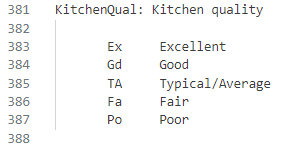
\includegraphics[width=0.4\textwidth]{figures/data_description.png} 
        \caption{Dataset Description Snapshot.}
        \label{fig:dataset_description_snapshot}
    \end{figure}
\end{frame}


% Slide 2-4: Dataset Samples and Statistics
\begin{frame}{Dataset Samples}
    \frametitle{Sample Data Overview}
    \begin{figure}
        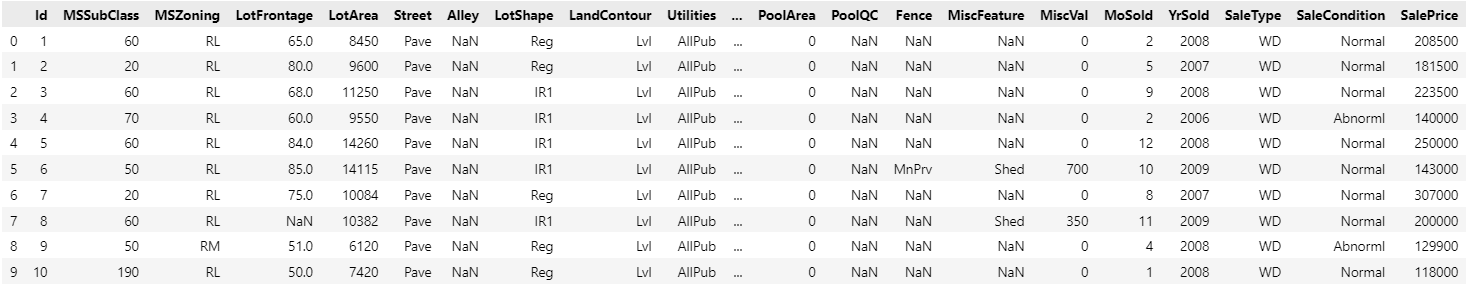
\includegraphics[width=1\textwidth]{figures/data_head.png} 
        \caption{Information of ten samples.}
        \label{fig:dataset_head}
    \end{figure}
\end{frame}

\begin{frame}{Correlation Matrix}
    \frametitle{Corralation Matrix}
    \begin{figure}
        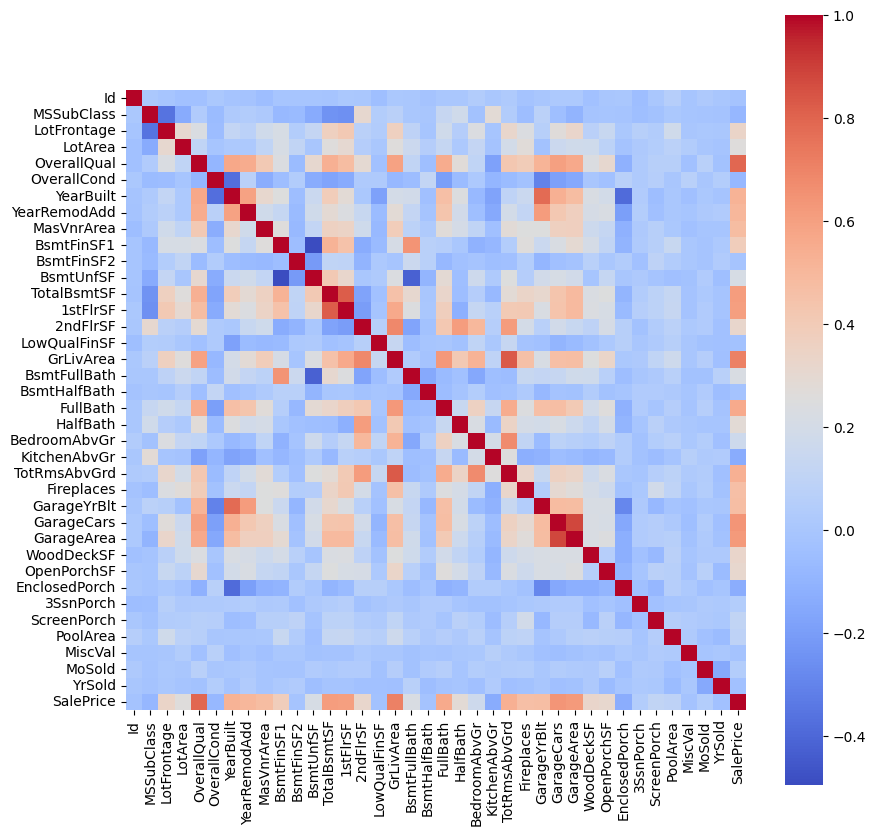
\includegraphics[width=0.55\textwidth]{figures/correlation_matrix.png} 
        \caption{Correlation Matrix Heat Map (Training Set).}
        \label{fig:correlation_matrix}
    \end{figure}
\end{frame}

\begin{frame}{Descriptive Statistics of SalePrice}
    \frametitle{Descriptive Statistics of SalePrice}
    \begin{table}[H]
        \centering
        \begin{tabular}{|l|r|}
        \hline
        \textbf{Statistic} & \textbf{Value} \\
        \hline
        Count & 1460 \\
        Mean & \$180,921.20 \\
        Standard Deviation & \$79,442.50 \\
        Minimum & \$34,900.00 \\
        25th Percentile & \$129,975.00 \\
        50th Percentile (Median) & \$163,000.00 \\
        75th Percentile & \$214,000.00 \\
        Maximum & \$755,000.00 \\
        \hline
        \end{tabular}
        \caption{Descriptive Statistics of \texttt{'SalePrice'} (Training Set).}
        \label{tab:saleprice_stats}
    \end{table}        
\end{frame}

% Slide 5: Handling Missing Values
\begin{frame}{Handling Missing Values}
    \frametitle{Imputing Data}
    \begin{itemize}
        \item Missing values in categorical columns imputed using the most frequent strategy.
        \item Done using \texttt{SimpleImputer} from scikit-learn with \texttt{strategy='most\_frequent'}.
        \item Missing values in numerical columns imputed using mean value.
        \item Done using \texttt{SimpleImputer} with \texttt{strategy='mean'} for numerical data.
        \item Applied the same transformation to both training and test datasets.
    \end{itemize}
\end{frame}

% Slide 6: Data Organization
\begin{frame}{Data Organization}
    \frametitle{Data Organization}
    \begin{itemize}
        \item Organized training data into feature matrix \(X_{\text{train}}\).
        \item Dropped \texttt{'SalePrice'} from feature matrix and assigned to target vector \(y_{\text{train}}\).
        \item Separated categorical and numerical columns for further processing.
    \end{itemize}
    \begin{table}[H]
        \centering
        \small
        \begin{tabular}{|l|c|}
        \hline
        \textbf{Column Type} & \textbf{Count} \\
        \hline
        Categorical Columns & 43 \\
        Numerical Columns & 36 \\
        \hline
        \end{tabular}
        \caption{Count of Categorical and Numerical Columns.}
        \label{tab:column_counts}
    \end{table}
\end{frame}

% Slide 7: Data Transformation Pipeline
\begin{frame}{Data Transformation Pipeline}
    \frametitle{Feature Encoding and Scaling}
    \begin{itemize}
        \item Applied one-hot encoding to categorical features to convert them into a numerical format.
        \item Standardized numerical features to have a mean of 0 and a standard deviation of 1.
        \item Used \texttt{ColumnTransformer} to apply these transformations in a composite manner.
        \item The processed data now ready for training machine learning models.
    \end{itemize}
\end{frame}

% Slide 8: Feature Selection with RFECV
\begin{frame}{Feature Selection with RFECV}
    \frametitle{Feature Selection Methodology}
    \begin{itemize}
        \item Employed Recursive Feature Elimination with Cross-Validation (RFECV) for feature selection.
        \item Used \texttt{XGBRFRegressor} as the estimator to assess feature importances.
        \item Linear Regression was choosen to predict the target variable.
        \item \texttt{RFECV} iteratively fits the model and removes the least significant features until the optimal number is achieved.
        \item Cross-validation with 5 folds was applied to ensure robust feature selection.
    \end{itemize}
\end{frame}

% Slide 9: RFECV Results
\begin{frame}{RFECV Results}
    \frametitle{Optimizing Feature Count}
    % \begin{itemize}
    %     \item The plot shows the model's performance on a specific number of features.
    %     \item Cross-validated R-squared score was used as the performance metric.
    % \end{itemize}
    % \vspace{0.5cm}
    \begin{figure}
        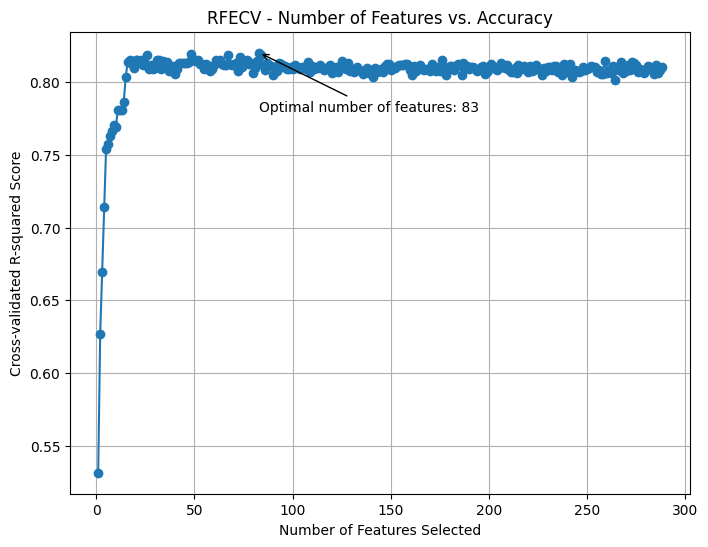
\includegraphics[width=0.7\textwidth]{figures/n_features_vs_score.png} 
        \caption{Number of Features vs. Cross-validated R-squared Score.}
        \label{fig:rfecv_plot}
    \end{figure}
\end{frame}

% Add more slides here describing the method of the feature extraction (As audience has no knowledge on that) and results

% Example frame 1
% \begin{frame}{frame} % set section name
%     \frametitle{frame}
%     \begin{itemize}
%         % Dataset Description
%         \item 1-2 slides
%         \item Describe the dataset (purpose, contents overview, creator, number of features, names of features…)
%         % Dataset Statistics
%         \item 3-5 slides
%         \item Present first couple of samples in the dataset
%         \item Present the statistics of the dataset, using both numerical and visualisation methods (please refer to the homework tasks)
%         % Data Engineering
%         \item 1-3 slides
%         \item Present what methods of data engineering you used in your work here (Missing values, Data cleaning, Data integration, Data standardization (normalization), Data transformation…)
%         \item Describe the reason and for using those methods
%         \item Present the effect of applying these methods
%     \end{itemize}
% \end{frame}